\begin{frame}{Monte-Carlo photon reconstruction efficiency}
\setlength{\unitlength}{1mm}
\begin{center}

\textcolor{blue}{\chibOneP}, \textcolor{red}{\chibTwoP}, \textcolor{cyan}{\chibThreeP} reconstruction efficiency in $\chib \to \Upsilon \gamma$ decays.

\begin{picture}(100,40)
      %
    \put(0,0){
      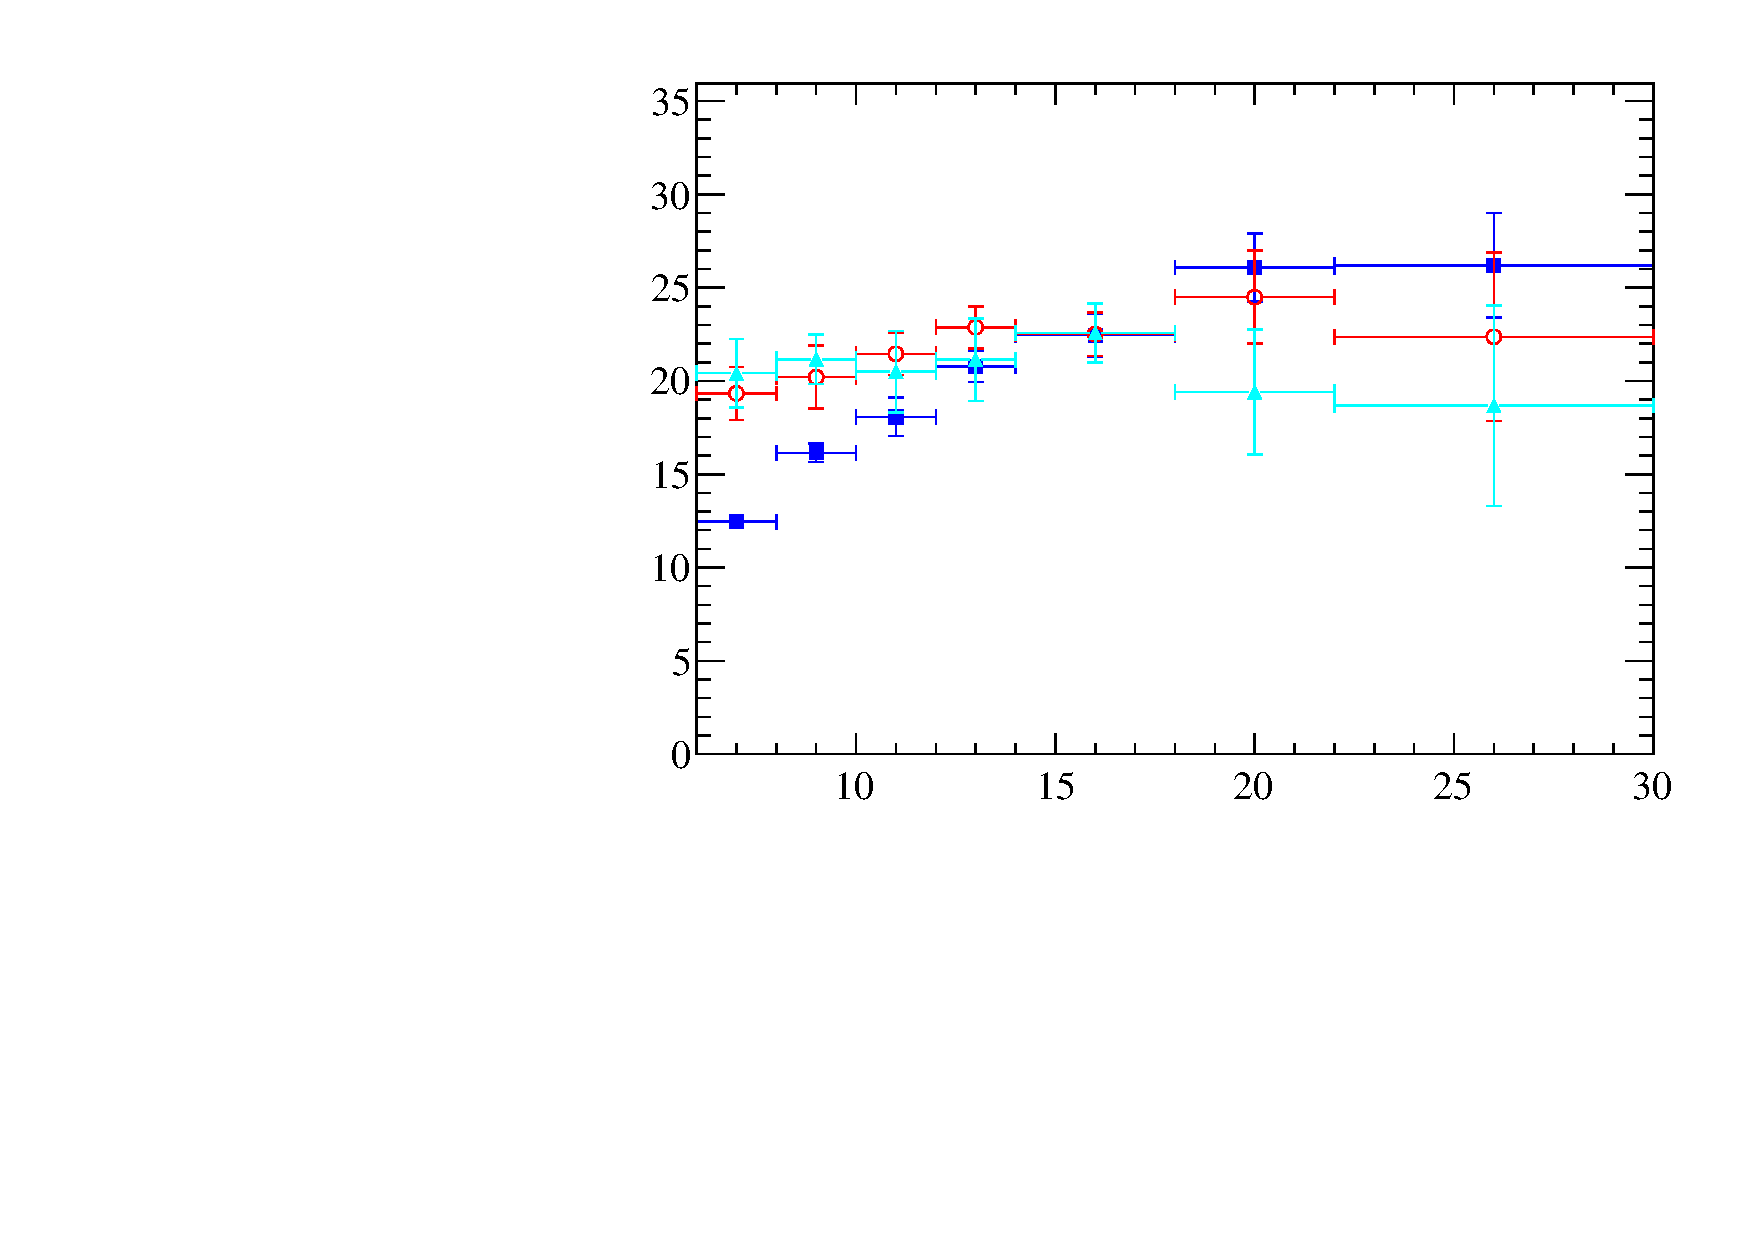
\includegraphics[width=50mm, height=40mm]{mc-eff/cb_ups1s}
    }
    \put(50,0){
      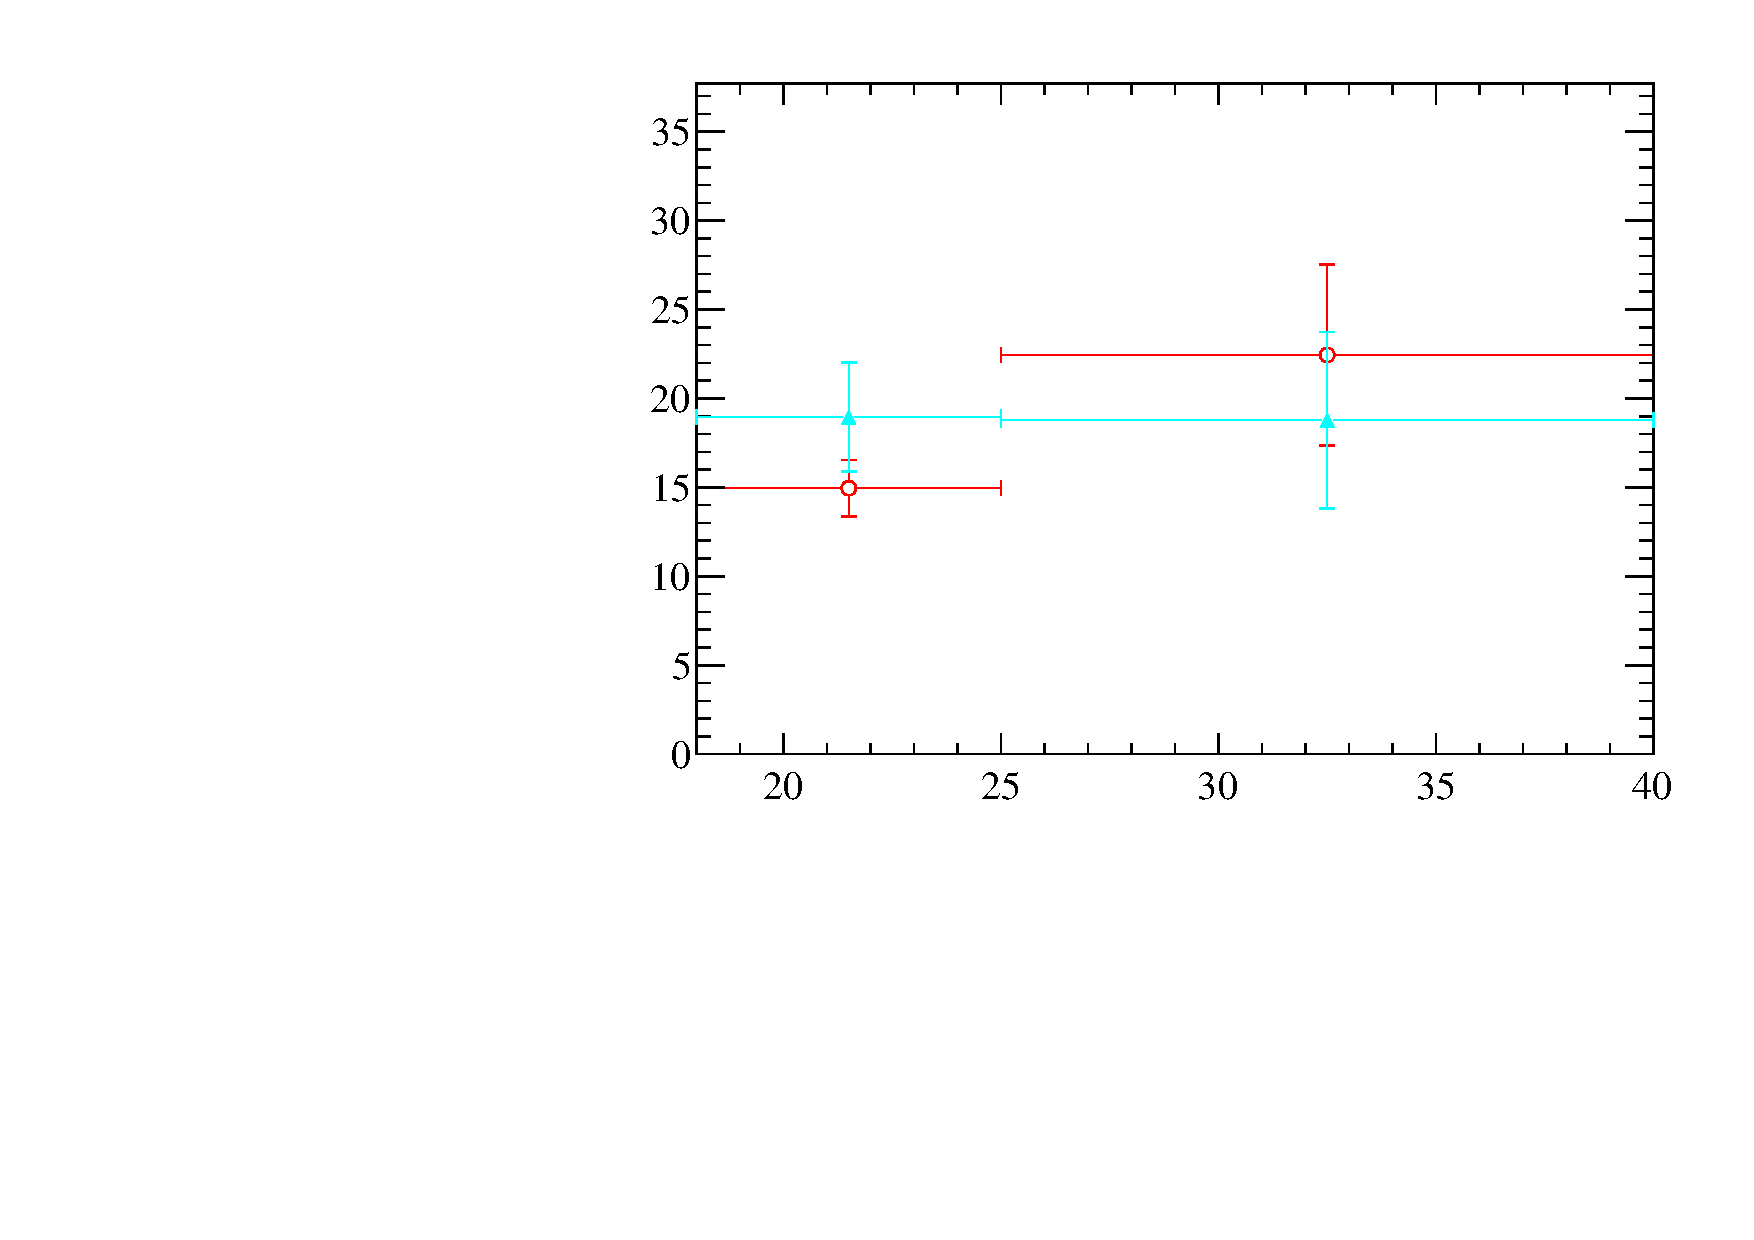
\includegraphics[width=50mm, height=40mm]{mc-eff/cb_ups2s}
    }
    
    \put(2,12){\begin{sideways}Efficiency (\%)\end{sideways}}
    \put(12,0){$p_T(\Y1S) \left[\gevcc\right]$}
    \put(10,35){\tiny $\chi_b(1,2,3P) \to \Y1S \gamma$}

    \put(52,12){\begin{sideways}Efficiency (\%)\end{sideways}}
    \put(62,0){$p_T(\Y2S) \left[\gevcc\right]$}
    \put(60,35){\tiny $\chi_b(2,3P) \to \Y2S \gamma$}


%    
%    \put(0,55){\tiny \begin{sideways}Candidates/(20\mevcc)\end{sideways}}
%    \put(2, 49.5){\tiny $m_{\mumu \gamma} - m_{\mumu} + 10.3552 \left[\gevcc\right]$}
%    \put(25,70){$\sqrt{s} = 7 \gev$}     
%    \graphpaper[2](0,0)(100, 40)        
  \end{picture}
 \end{center}
\begin{block}{}
Photons is more energetic as $p_T(\Upsilon)$ increases so it is reconstructed more efficiently.
\end{block}

\end{frame}